\documentclass[11pt]{article} % use larger type; default would be 10pt

\usepackage{pgfplots}
\usetikzlibrary{calc}
\usetikzlibrary{arrows}
\usetikzlibrary{patterns}
\usetikzlibrary{calc,intersections,through,backgrounds}
\usetikzlibrary{decorations.pathreplacing}
        \newcommand\degree[0]{^{\circ}}
        \newcommand\abs[1]{\left|#1\right|}

\title{Play with TikZ}
\author{Just Us}
%\date{} % Activate to display a given date or no date (if empty),
         % otherwise the current date is printed 

\begin{document}
\maketitle

\section{Chap 9 Vectors}

\subsection{9.2 Coordinate form}




exam9-2-1

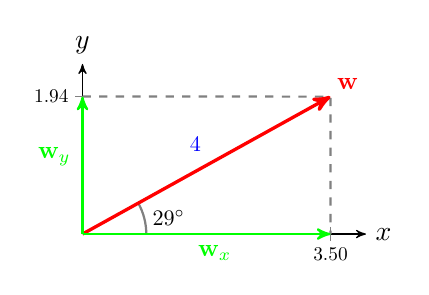
\begin{tikzpicture} [scale=.9]
\draw[black,->,>=stealth'] (0,0)--(4.,0) node[right] {$x$};
\draw[black,->,>=stealth'] (0,0)--(0,2.4) node[above] {$y$};
\coordinate (w) at (29:4);
\coordinate (wx) at (3.5,0);
\coordinate (wy) at (0, 1.94);

\draw[gray] (3.5,.1)--++(0, -.2) node[below, text=black, scale=.7]{3.50};
\draw[gray] (.1, 1.94)--++(-.2, 0) node[left, text=black, scale=.7]{1.94};
\node[text width=.3cm, text=blue, scale=.8] at ($ .5*(w) + (-.1, .3) $) {4};

\draw[gray, thick] (0.9,0) arc (0:29:0.9) node[right, midway, text=black, scale=.8] {$29\degree$};
\draw[gray, thick, dashed] (wy)--(w)--(wx);
\draw[red, very thick,->,>=stealth'] (0,0)--++(w) node[above right, xshift=1,  yshift=1, scale=.9, fill=white, inner sep=1]{\textbf{w}};
\draw[green, thick,->,>=stealth'] (0,0)--++(wx) node[below, midway, xshift=3, yshift=-3, scale=.9, fill=white, inner sep=1]{$\textbf{w}_x$};
\draw[green, thick,->,>=stealth'] (0,0)--++(wy) node[left, midway, xshift=-3, yshift=3, scale=.9, fill=white, inner sep=1]{$\textbf{w}_y$};


\end{tikzpicture}
\newline


fig9-2-1

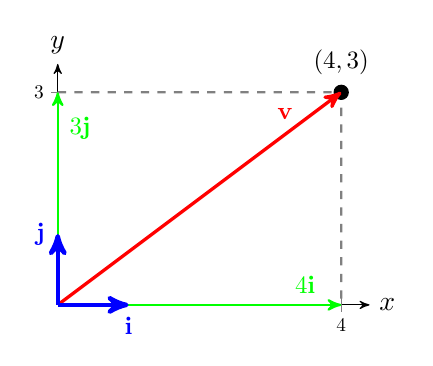
\begin{tikzpicture} [scale=.9]
\draw[black,->,>=stealth'] (0,0)--(4.4,0) node[right] {$x$};
\draw[black,->,>=stealth'] (0,0)--(0,3.4) node[above] {$y$};
\coordinate (O) at (0,0);
\coordinate (v) at (4,3);
\coordinate (wx) at (4,0);
\coordinate (wy) at (0, 3);
\coordinate (i) at (1,0);
\coordinate (j) at (0,1);

\draw[gray] (4,.1)--++(0, -.2) node[below, text=black, scale=.7]{4};
\draw[gray] (.1, 3)--++(-.2, 0) node[left, text=black, scale=.7]{3};
\draw[gray, thick, dashed] (0,3)--(v)--(4,0);
\filldraw[black] (v) circle (.1) node[above, yshift=3, scale=.9]{$(4,3)$};

\draw[red, very thick,->,>=stealth'] (O)--++(v) node[left, xshift=-16,  yshift=-8, scale=.9, fill=white, inner sep=1]{\textbf{v}};
\draw[green, thick,->,>=stealth'] (O)--++(4,0) node[above, xshift=-13, yshift=3, scale=.9, fill=white, inner sep=1]{$4\textbf{i}$};
\draw[green, thick,->,>=stealth'] (O)--++(0,3) node[right, xshift=3, yshift=-13, scale=.9, fill=white, inner sep=1]{$3\textbf{j}$};
\draw[blue, ultra thick,->,>=stealth'] (O)--++(i) node[below, yshift=-3, scale=.9, fill=white, inner sep=1]{$\textbf{i}$};
\draw[blue, ultra thick,->,>=stealth'] (O)--++(j) node[left, xshift=-3, scale=.9, fill=white, inner sep=1]{$\textbf{j}$};

\end{tikzpicture}
\newline


exam9-2-2

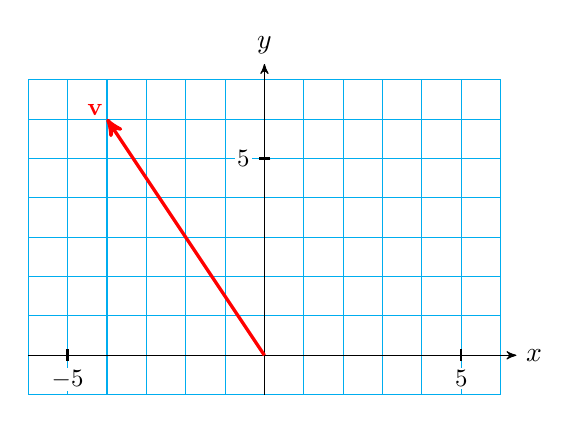
\begin{tikzpicture} [scale=.5]
\draw[cyan] (-6,-1) grid (6,7);
\draw[black,->,>=stealth'] (-6,0)--(6.4,0) node[right] {$x$};
\draw[black,->,>=stealth'] (0,-1)--(0,7.4) node[above] {$y$};
\foreach \x   in  {5} {
 \draw[black, thick] (\x,0.15) --++(0,-.3) node[below, yshift=-2, fill=white, inner sep=1, scale=.9] {$\x$};
 \draw[black, thick] (-\x,0.15) --++(0,-.3) node[below, yshift=-2, fill=white, inner sep=1, scale=.9] {$-\x$};
 \draw[black, thick] (0.15,\x) --++(-.3,0) node[left, xshift=-2, fill=white, inner sep=1, scale=.9] {$\x$};
};
\coordinate (O) at (0,0);
\coordinate (v) at (-4,6);

\draw[red, very thick,->,>=stealth'] (O)--++(v) node[above left, scale=.9, fill=white, inner sep=1]{\textbf{v}};

\end{tikzpicture}
\newline


exer9-2-2

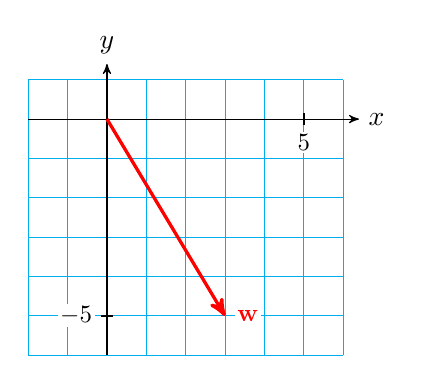
\begin{tikzpicture} [scale=.5]
\draw[cyan] (-2,-6) grid (6,1);
\draw[black,->,>=stealth'] (-2,0)--(6.4,0) node[right] {$x$};
\draw[black,->,>=stealth'] (0,-6)--(0,1.4) node[above] {$y$};
\foreach \x   in  {5} {
 \draw[black, thick] (\x,0.15) --++(0,-.3) node[below, yshift=-2, fill=white, inner sep=1, scale=.9] {$\x$};
 \draw[black, thick] (0.15,-\x) --++(-.3,0) node[left, xshift=-2, fill=white, inner sep=1, scale=.9] {$-\x$};
};
\coordinate (O) at (0,0);
\coordinate (v) at (3,-5);

\draw[red, very thick,->,>=stealth'] (O)--++(v) node[right, xshift=3, scale=.9, fill=white, inner sep=1]{\textbf{w}};

\end{tikzpicture}
\newline



fig9-2-2

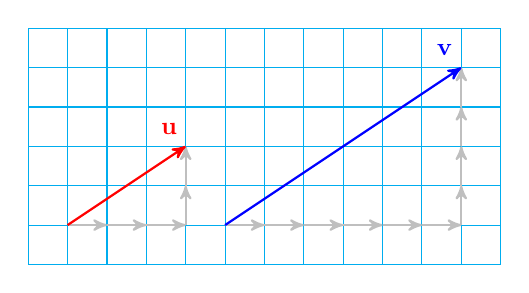
\begin{tikzpicture} [scale=.5]
\draw[cyan] (0,0) grid (12,6);

\coordinate (u) at (3,2);
\coordinate (v) at ($ 2*(u) $);
\coordinate (i) at (1,0);
\coordinate (j) at (0,1);

\foreach \x in {1, 2, 3, 5, 6, 7, 8, 9,10} {
 \draw[lightgray, thick, ->,>=stealth'] (\x,1)--++(i);
};

\foreach \y in {1, 2} {
 \draw[lightgray, thick, ->,>=stealth'] (4,\y)--++(j);
};
\foreach \y in {1,2,3,4} {
 \draw[lightgray, thick, ->,>=stealth'] (11,\y)--++(j);
};

\draw[red, thick,->,>=stealth'] (1,1)--++(u) node[above, xshift=-6, yshift=3, scale=.9, fill=white, inner sep=1]{\textbf{u}};
\draw[blue, thick,->,>=stealth'] (5,1)--++(v) node[above, xshift=-6, yshift=3, scale=.9, fill=white, inner sep=1]{\textbf{v}};

\end{tikzpicture}
\newline



fig9-2-3a


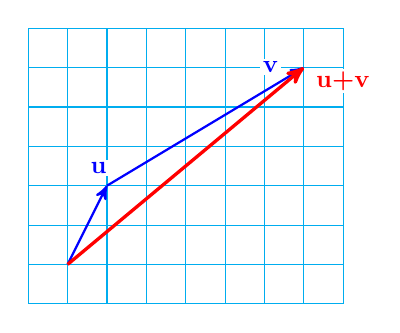
\begin{tikzpicture} [scale=.5]
\draw[cyan] (0,0) grid (8,7);

\coordinate (u) at (1,2);
\coordinate (v) at (5,3);
\coordinate (s) at ($ (u) + (v) $);

\draw[blue, thick,->,>=stealth'] (1,1)--++(u) node[above, xshift=-3, yshift=3, scale=.9, fill=white, inner sep=1]{\textbf{u}};
\draw[blue, thick,->,>=stealth'] (2,3)--++(v) node[above, xshift=-12, yshift=-3, scale=.9, fill=white, inner sep=1]{\textbf{v}};
\draw[red, very thick,->,>=stealth'] (1,1)--++(s) node[right, xshift=3, yshift=-5, scale=.9, fill=white, inner sep=1]{\textbf{u+v}};

\end{tikzpicture}
\newline



fig9-2-3b

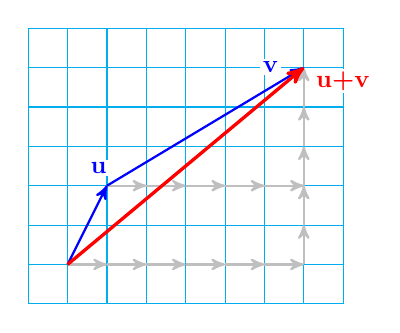
\begin{tikzpicture} [scale=.5]
\draw[cyan] (0,0) grid (8,7);

\coordinate (u) at (1,2);
\coordinate (v) at (5,3);
\coordinate (s) at ($ (u) + (v) $);
\coordinate (i) at (1,0);
\coordinate (j) at (0,1);

 \draw[lightgray, thick, ->,>=stealth'] (1,1)--++(i);
\foreach \x in { 2, 3, 4, 5, 6} {
 \draw[lightgray, thick, ->,>=stealth'] (\x,1)--++(i);
 \draw[lightgray, thick, ->,>=stealth'] (\x,3)--++(i);
};

\foreach \y in {1,2,3,4, 5} {
 \draw[lightgray, thick, ->,>=stealth'] (7,\y)--++(j);
};

\draw[blue, thick,->,>=stealth'] (1,1)--++(u) node[above, xshift=-3, yshift=3, scale=.9, fill=white, inner sep=1]{\textbf{u}};
\draw[blue, thick,->,>=stealth'] (2,3)--++(v) node[above, xshift=-12, yshift=-3, scale=.9, fill=white, inner sep=1]{\textbf{v}};
\draw[red, very thick,->,>=stealth'] (1,1)--++(s) node[right, xshift=3, yshift=-5, scale=.9, fill=white, inner sep=1]{\textbf{u+v}};

\end{tikzpicture}
\newline





fig9-2-3

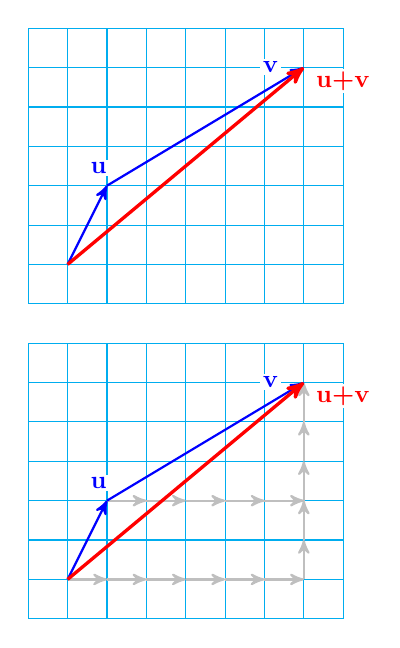
\begin{tikzpicture} [scale=.5]
\draw[cyan] (0,0) grid (8,7);

\coordinate (u) at (1,2);
\coordinate (v) at (5,3);
\coordinate (s) at ($ (u) + (v) $);

\draw[blue, thick,->,>=stealth'] (1,1)--++(u) node[above, xshift=-3, yshift=3, scale=.9, fill=white, inner sep=1]{\textbf{u}};
\draw[blue, thick,->,>=stealth'] (2,3)--++(v) node[above, xshift=-12, yshift=-3, scale=.9, fill=white, inner sep=1]{\textbf{v}};
\draw[red, very thick,->,>=stealth'] (1,1)--++(s) node[right, xshift=3, yshift=-5, scale=.9, fill=white, inner sep=1]{\textbf{u+v}};

%second grid
\coordinate (O) at (0,-8);

\draw[cyan] (O) grid ($ (O)+(8,7) $);

\coordinate (i) at (1,0);
\coordinate (j) at (0,1);

 \draw[lightgray, thick, ->,>=stealth'] ($ (O)+(1,1) $)--++(i);
\foreach \x in { 2, 3, 4, 5, 6} {
 \draw[lightgray, thick, ->,>=stealth']  ($ (O)+(\x,1)$)--++(i);
 \draw[lightgray, thick, ->,>=stealth']  ($ (O)+(\x,3) $)--++(i);
};

\foreach \y in {1,2,3,4, 5} {
 \draw[lightgray, thick, ->,>=stealth']  ($ (O)+(7,\y)$)--++(j);
};

\draw[blue, thick,->,>=stealth']  ($ (O)+(1,1)$)--++(u) node[above, xshift=-3, yshift=3, scale=.9, fill=white, inner sep=1]{\textbf{u}};
\draw[blue, thick,->,>=stealth']  ($ (O)+(2,3)$)--++(v) node[above, xshift=-12, yshift=-3, scale=.9, fill=white, inner sep=1]{\textbf{v}};
\draw[red, very thick,->,>=stealth']  ($ (O)+(1,1)$)--++(s) node[right, xshift=3, yshift=-5, scale=.9, fill=white, inner sep=1]{\textbf{u+v}};

\end{tikzpicture}
\newline



exam9-2-6

\begin{tikzpicture} [scale=.15]

\coordinate (O) at (0,0);
\coordinate (v) at (225:15);
\coordinate (w) at (190:20);
\coordinate (s) at ($ (u) + (v) $);
\def\u{4};

\coordinate (i) at (\u,0);
\coordinate (j) at (0,\u);

\draw[lightgray, thick, ->,>=stealth'] (O)--++(i);
\draw[lightgray, thick, ->,>=stealth'] (O)--++(j);
\draw[lightgray, thick, ->,>=stealth'] (v)--++(i);
\draw[lightgray, thick, ->,>=stealth'] (v)--++(j);

\draw[lightgray, thick, ->,>=stealth'] (1.5,0)arc (0:225: 1.5) node[above left, midway, yshift=-5, scale=0.8, text=black]{$225\degree$};
\draw[lightgray, thick, ->,>=stealth'] ($ (v)+(1.5,0)$) arc (0:190: 1.5) node[above left, midway, yshift=-5, scale=0.8, text=black]{$190\degree$};
\draw[lightgray, thick, ->,>=stealth'] ($ (v)+(0,2)$) arc (90:-170: 2) node[below right, midway, xshift=-5, scale=0.8, text=black]{$260\degree$};

\draw[red, thick,->,>=stealth'] (O)--++(v) node[below right, midway, xshift=3, scale=.9, fill=white, inner sep=1, text=blue]{15 mi};
\draw[red, thick,->,>=stealth'] (v)--++(w) node[below, midway , xshift=-2, yshift=-5, scale=.9, fill=white, inner sep=1, text=blue]{20 mi};

\end{tikzpicture}
\newline


exer9-2-7ans

\begin{tikzpicture} [scale=2]
\coordinate (O) at (0,0);
\coordinate (v) at (-85:1.6);
\coordinate (w) at (25:0.8);
\coordinate (x) at (100:1.2);
\coordinate (s) at ($ (u) + (v) $);
\def\u{0.5};

\coordinate (i) at (\u,0);
\coordinate (j) at (0,\u);

\draw[lightgray, thick, ->,>=stealth'] (O)--++($.7*(j)$);
\draw[lightgray, thick, <->,>=stealth'] (0,.15) arc (90:-85: 0.15) node[right, midway, yshift=-1, scale=0.8, text=black]{$175\degree$};
\draw[lightgray, thick, ->,>=stealth'] ($(v)+(w)$)--++(j);
\draw[lightgray, thick, <-,>=stealth'] ($(v)+(w)+(0,.3)$) arc (90:60: 0.3) node[right, xshift=-1, yshift=-1, scale=0.8, text=black]{$10\degree$};
\draw[lightgray, thick, <-,>=stealth'] ($(v)+(w)+0.25*(x)$) arc (95:125: 0.35) ;
\draw[lightgray, thick, ->,>=stealth'] (v)--++(j);
\draw[lightgray, thick, <->,>=stealth'] ($(v)+(0,.3)$) arc (90:25: 0.3) node[above right, midway, xshift=-2, yshift=-1, scale=0.8, text=black]{$65\degree$};

\draw[red, thick,->,>=stealth'] (O)--++(v) node[left, midway, xshift=-3, scale=.9, fill=white, inner sep=1, text=blue]{1.6 km};
\draw[red, thick,->,>=stealth'] (v)--++(w) node[below, midway, xshift=6, yshift=-5, scale=.9, fill=white, inner sep=1, text=blue]{0.8 km};
\draw[red, thick,->,>=stealth'] ($(v)+(w)$)--++(x) node[left, midway , xshift=-2, yshift=-5, scale=.9, fill=white, inner sep=1, text=blue]{1.2 km};

\end{tikzpicture}
\newline


exam9-2-8

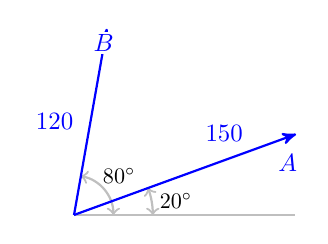
\begin{tikzpicture} [scale=0.02]
\coordinate (O) at (0,0);
\coordinate (A) at (20:150);
\coordinate (B) at (80:120);

\draw[lightgray, thick] (O)--++(140,0);
\draw[lightgray, thick, <->] (50,0) arc (0:20: 50) node[right, midway, scale=0.8, text=black]{$20\degree$};
\draw[lightgray, thick, <->] (25,0) arc (0:80: 25) node[right, xshift=3, xshift=2, scale=0.8, text=black]{$80\degree$};

\draw[blue, thick,->,>=stealth'] (O)--++(A) node[below, xshift=-3, yshift=-6, scale=.9, fill=white, inner sep=1, text=blue]{$A$};
\draw[blue, thick,->,>=stealth'] (O)--++(B) node[right, xshift=-6, yshift=-5, scale=.9, fill=white, inner sep=1, text=blue]{$B$};
\node[left, xshift=-3, scale=.9, text=blue] at ($ .5*(B) $) {120};
\node[left, yshift=6, scale=.9, text=blue] at ($ .8*(A) $) {150};

\end{tikzpicture}
\newline


exam9-2-8ans

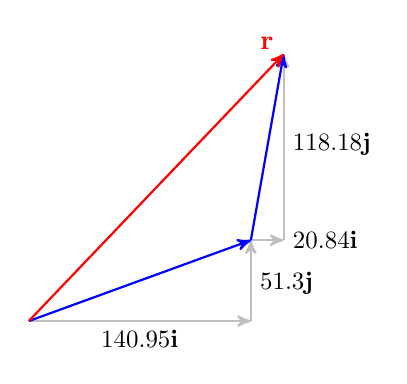
\begin{tikzpicture} [scale=0.02]
\coordinate (O) at (0,0);
\coordinate (A) at (20:150);
\coordinate (B) at (80:120);
\coordinate (r) at ($ (A) + (B) $);
\coordinate (Ax) at ($ 150*cos(20)*(1,0)  $);
\coordinate (Ay) at ($ 150*sin(20)*(0,1)  $);
\coordinate (Bx) at ($ 120*cos(80)*(1,0)  $);
\coordinate (By) at ($ 120*sin(80)*(0,1)  $);

\draw[lightgray, thick, ->, >=stealth'] (O)--++(Ax) node[below, midway, scale=.9, text=black]{140.95\textbf{i}};
\draw[lightgray, thick, ->, >=stealth'] (Ax)--++(Ay) node[right, midway, yshift=-1, scale=.9, text=black]{51.3\textbf{j}};
\draw[lightgray, thick, ->, >=stealth'] (A)--++(Bx) node[right, scale=.9, text=black]{20.84\textbf{i}};
\draw[lightgray, thick, ->, >=stealth'] ($ (A) +(Bx)$)--++(By) node[right, midway, yshift=1, scale=.9, text=black]{118.18\textbf{j}};

\draw[blue, thick,->,>=stealth'] (O)--++(A);
\draw[blue, thick,->,>=stealth'] (A)--++(B) ;
\draw[red, thick,->,>=stealth'] (O)--++(r) node[above left, yshift=-2] {\textbf{r}};

\end{tikzpicture}
\newline


hp9-2-1

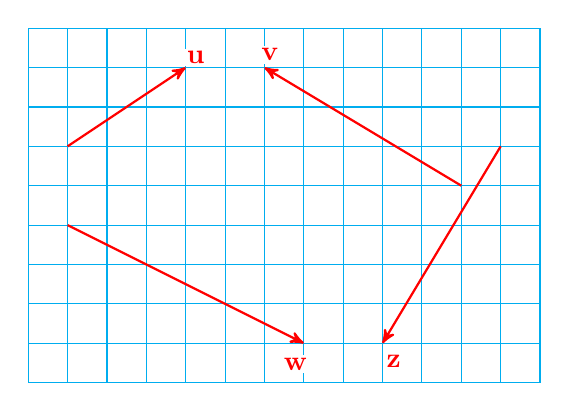
\begin{tikzpicture} [scale=0.5]

\draw[cyan] (0,0) grid (13,9);
\coordinate (u) at (3,2);
\coordinate (v) at (-5,3);
\coordinate (w) at (6,-3);
\coordinate (z) at (-3, -5);

\draw[red, thick,->,>=stealth'] (1,6)--++(u) node[above right, xshift=-1, fill=white, inner sep=1] {\textbf{u}};
\draw[red, thick,->,>=stealth'] (11,5)--++(v) node[above , xshift=2, yshift=1, fill=white, inner sep=1] {\textbf{v}};;
\draw[red, thick,->,>=stealth'] (1,4)--++(w) node[ below, xshift=-3, yshift=-4, fill=white, inner sep=1] {\textbf{w}};
\draw[red, thick,->,>=stealth'] (12,6)--++(z) node[below, xshift=4, yshift=-3, fill=white, inner sep=1] {\textbf{z}};

\end{tikzpicture}
\newline



hp9-2-7

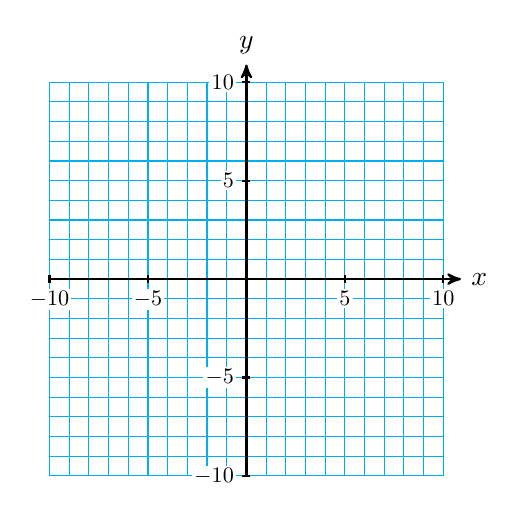
\begin{tikzpicture} [scale=0.25]

\draw[cyan] (-10,-10) grid (10,10);
\draw[black, thick,->,>=stealth'] (-10,0)--(10.9,0) node[right] {$x$};
\draw[black, thick,->,>=stealth'] (0,-10)--(0,10.9) node[above] {$y$};

\foreach \x in {-10,-5,5,10} {
 \draw[black,thick] (\x,0.2)--++(0,-.4) node[below, yshift=-2, scale=.8, fill=white, inner sep=1]{$\x$};
 \draw[black,thick] (0.2,\x)--++(-.4,0) node[left, xshift=-2, scale=.8, fill=white, inner sep=1]{$\x$};
}

\end{tikzpicture}
\newline



hp9-2-7ans

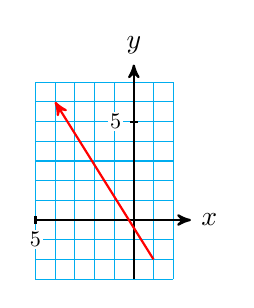
\begin{tikzpicture} [scale=0.25]

\draw[cyan] (-5,-3) grid (2,7);
\draw[black, thick,->,>=stealth'] (-5,0)--(2.9,0) node[right] {$x$};
\draw[black, thick,->,>=stealth'] (0,-3)--(0,7.9) node[above] {$y$};

\foreach \x in {5} {
 \draw[black,thick] (-\x,0.2)--++(0,-.4) node[below, yshift=-2, scale=.8, fill=white, inner sep=1]{$\x$};
 \draw[black,thick] (0.2,\x)--++(-.4,0) node[left, xshift=-2, scale=.8, fill=white, inner sep=1]{$\x$};
}

\draw[red, thick,->,>=stealth'] (1,-2)--(-4,6);

\end{tikzpicture}
\newline



hp9-2-9ans
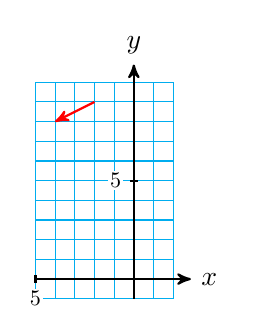
\begin{tikzpicture} [scale=0.25]
\draw[cyan] (-5,-1) grid (2,10);
\draw[black, thick,->,>=stealth'] (-5,0)--(2.9,0) node[right] {$x$};
\draw[black, thick,->,>=stealth'] (0,-1)--(0,10.9) node[above] {$y$};

\foreach \x in {5} {
 \draw[black,thick] (-\x,0.2)--++(0,-.4) node[below, yshift=-2, scale=.8, fill=white, inner sep=1]{$\x$};
 \draw[black,thick] (0.2,\x)--++(-.4,0) node[left, xshift=-2, scale=.8, fill=white, inner sep=1]{$\x$};
}

\draw[red, thick,->,>=stealth'] (-2,9)--(-4,8);

\end{tikzpicture}
\newline



hp9-2-23ans
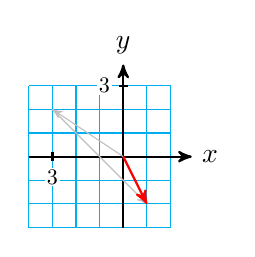
\begin{tikzpicture} [scale=0.3]
\draw[cyan] (-4,-3) grid (2,3);
\draw[black, thick,->,>=stealth'] (-4,0)--(2.9,0) node[right] {$x$};
\draw[black, thick,->,>=stealth'] (0,-3)--(0,3.9) node[above] {$y$};

\foreach \x in {3} {
 \draw[black,thick] (-\x,0.2)--++(0,-.4) node[below, yshift=-2, scale=.8, fill=white, inner sep=1]{$\x$};
 \draw[black,thick] (0.2,\x)--++(-.4,0) node[left, xshift=-2, scale=.8, fill=white, inner sep=1]{$\x$};
}

\coordinate(u) at (-3,2);
\coordinate(v) at (4,-4);

\draw[lightgray,->,>=stealth'] (0,0)--(u);
\draw[lightgray,->,>=stealth'] (u)--++(v);
\draw[red, thick,->,>=stealth'] (0,0)--($ (u)+(v)$);

\end{tikzpicture}
\newline



hp9-2-25ans
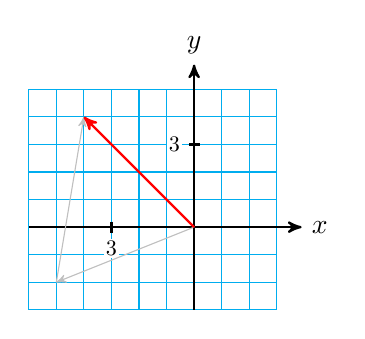
\begin{tikzpicture} [scale=0.35]
\draw[cyan] (-6,-3) grid (3,5);
\draw[black, thick,->,>=stealth'] (-6,0)--(3.9,0) node[right] {$x$};
\draw[black, thick,->,>=stealth'] (0,-3)--(0,5.9) node[above] {$y$};

\foreach \x in {3} {
 \draw[black,thick] (-\x,0.2)--++(0,-.4) node[below, yshift=-2, scale=.8, fill=white, inner sep=1]{$\x$};
 \draw[black,thick] (0.2,\x)--++(-.4,0) node[left, xshift=-2, scale=.8, fill=white, inner sep=1]{$\x$};
}

\coordinate(u) at (-5,-2);
\coordinate(v) at (1,6);

\draw[lightgray,->,>=stealth'] (0,0)--(u);
\draw[lightgray,->,>=stealth'] (u)--++(v);
\draw[red, thick,->,>=stealth'] (0,0)--($ (u)+(v)$);

\end{tikzpicture}
\newline



hp9-2-2-47ans
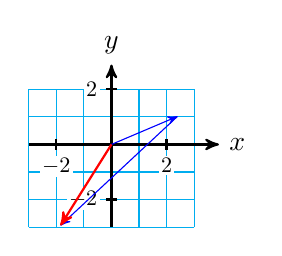
\begin{tikzpicture} [scale=0.35]
\draw[cyan] (-3,-3) grid (3,2);
\draw[black, thick,->,>=stealth'] (-3,0)--(3.9,0) node[right] {$x$};
\draw[black, thick,->,>=stealth'] (0,-3)--(0,2.9) node[above] {$y$};

\foreach \x in {2} {
 \draw[black,thick] (\x,0.2)--++(0,-.4) node[below, yshift=-2, scale=.8, fill=white, inner sep=1]{$\x$};
 \draw[black,thick] (0.2,\x)--++(-.4,0) node[left, xshift=-2, scale=.8, fill=white, inner sep=1]{$\x$};
 \draw[black,thick] (-\x,0.2)--++(0,-.4) node[below, yshift=-2, scale=.8, fill=white, inner sep=1]{$-\x$};
 \draw[black,thick] (0.2,-\x)--++(-.4,0) node[left, xshift=-2, scale=.8, fill=white, inner sep=1]{$-\x$};
}

\coordinate(u) at (23:2.6);
\coordinate(v) at (223:5.8);

\draw[blue,->,>=stealth'] (0,0)--(u);
\draw[blue,->,>=stealth'] (u)--++(v);
\draw[red, thick,->,>=stealth'] (0,0)--($ (u)+(v)$);

\end{tikzpicture}
\newline



hp9-2-2-49ans
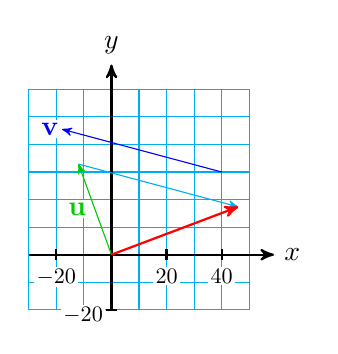
\begin{tikzpicture} [scale=0.035]
\draw[cyan] (-30,-20) grid[step=10] (50,60);
\draw[black, thick,->,>=stealth'] (-30,0)--(59,0) node[right] {$x$};
\draw[black, thick,->,>=stealth'] (0,-20)--(0,69) node[above] {$y$};

 \draw[black,thick] (40,02)--++(0,-4) node[below, yshift=-2, scale=.8, fill=white, inner sep=1]{$40$};

\foreach \x in {20} {
 \draw[black,thick] (\x,02)--++(0,-4) node[below, yshift=-2, scale=.8, fill=white, inner sep=1]{$\x$};
 \draw[black,thick] (-\x,02)--++(0,-4) node[below, yshift=-2, scale=.8, fill=white, inner sep=1]{$-\x$};
 \draw[black,thick] (2,-\x)--++(-4,0) node[left, yshift=-2, scale=.8, fill=white, inner sep=1]{$-\x$};
}

\coordinate(u) at (110:35);
\coordinate(v) at (165:60);

\draw[green!80!black,->,>=stealth'] (0,0)--(u) node[left,midway, xshift=-2, fill=white, inner sep=1]{\textbf{u}};
%\draw[blue,->,>=stealth'] (u)--++(v);
\draw[blue,->,>=stealth'] (40,30)--++(v) node[left, fill=white, inner sep=1]{\textbf{v}};
\draw[cyan,->,>=stealth'] (u)--++($-1*(v)$);
\draw[red, thick,->,>=stealth'] (0,0)--($ (u)-(v)$);

\end{tikzpicture}
\newline



hp9-2-2-51ans
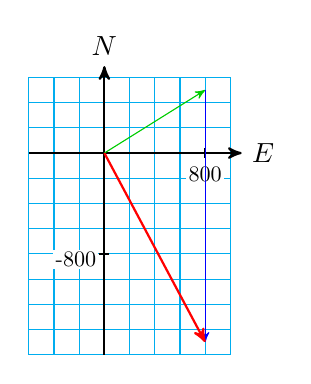
\begin{tikzpicture} [scale=.16]
\draw[cyan] (-6,-16) grid[step=2] (10,6);
\draw[black, thick,->,>=stealth'] (-6,0)--(10.9,0) node[right] {$E$};
\draw[black, thick,->,>=stealth'] (0,-16)--(0,6.90) node[above] {$N$};

\draw[black,thick] (8,.40)--++(0,-.80) node[below, yshift=-2, scale=.8, fill=white, inner sep=1]{$800$};
\draw[black,thick] (.40,-8)--++(-.80,0) node[left, yshift=-2, scale=.8, fill=white, inner sep=1]{-$800$};

\coordinate(u) at (8,5);
\coordinate(v) at (0,-20);

\draw[green!80!black,->,>=stealth'] (0,0)--(u);
\draw[blue,->,>=stealth'] (u)--++(v);
\draw[red, thick,->,>=stealth'] (0,0)--($ (u)+(v)$);

\end{tikzpicture}
\newline



hp9-2-2-53ans
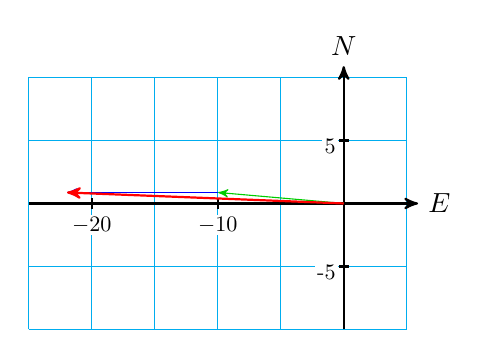
\begin{tikzpicture} [scale=.16]
\draw[cyan] (-25,-10) grid[step=5] (5,10);
\draw[black, thick,->,>=stealth'] (-25,0)--(5.9,0) node[right] {$E$};
\draw[black, thick,->,>=stealth'] (0,-10)--(0,10.90) node[above] {$N$};

\draw[black,thick] (-10,.40)--++(0,-.80) node[below, yshift=-2, scale=.8, fill=white, inner sep=1]{$-10$};
\draw[black,thick] (-20,.40)--++(0,-.80) node[below, yshift=-2, scale=.8, fill=white, inner sep=1]{$-20$};
\draw[black,thick] (.40,-5)--++(-.80,0) node[left, yshift=-2, scale=.8, fill=white, inner sep=1]{-$5$};
\draw[black,thick] (.40,5)--++(-.80,0) node[left, yshift=-2, scale=.8, fill=white, inner sep=1]{$5$};

\coordinate(u) at (175:10);
\coordinate(v) at (180:12);

\draw[green!80!black,->,>=stealth'] (0,0)--(u);
\draw[blue,->,>=stealth'] (u)--++(v);
\draw[red, thick,->,>=stealth'] (0,0)--($ (u)+(v)$);

\end{tikzpicture}
\newline



hp9-2-2-55ans
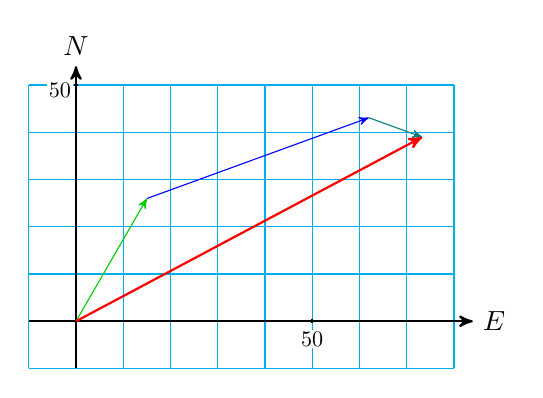
\begin{tikzpicture} [scale=.06]
\draw[cyan] (-10,-10) grid[step=10] (80,50);
\draw[black, thick,->,>=stealth'] (-10,0)--(84,0) node[right] {$E$};
\draw[black, thick,->,>=stealth'] (0,-10)--(0,54) node[above] {$N$};

\draw[black,thick] (50,.40)--++(0,-.80) node[below, yshift=-2, scale=.8, fill=white, inner sep=1]{$50$};
\draw[black,thick] (.40,50)--++(-.80,0) node[left, yshift=-2, scale=.8, fill=white, inner sep=1]{$50$};

\coordinate(u) at (60:30);
\coordinate(v) at (20:50);
\coordinate(w) at (-20:12);

\draw[green!80!black,->,>=stealth'] (0,0)--(u);
\draw[blue,->,>=stealth'] (u)--++(v);
\draw[teal,->,>=stealth'] ($ (u)+(v)$)--++(w);
\draw[red, thick,->,>=stealth'] (0,0)--($ (u)+(v)+(w)$);

\end{tikzpicture}
\newline



hp9-2-2-59
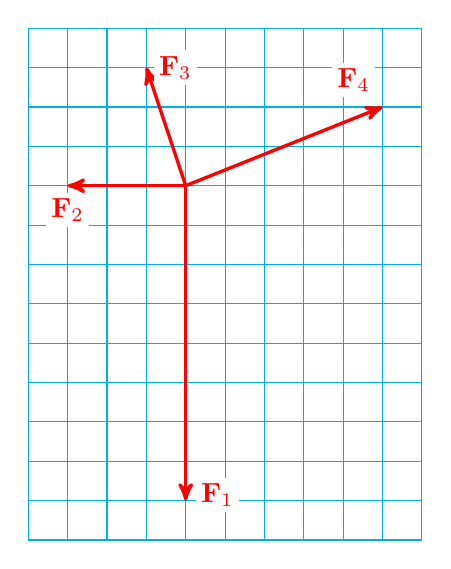
\begin{tikzpicture} [scale=.5]
\draw[cyan] (0,0) grid (10,13);

\coordinate(O) at (4,9);
\coordinate(f1) at (0,-8);
\coordinate(f2) at (-3,0);
\coordinate(f3) at (-1,3);
\coordinate(f4) at (5,2);

\draw[red, very thick,->,>=stealth'] (O)--++(f1) node[right, xshift=3, yshift=2, fill=white, inner sep = 2]{$\textbf{F}_1$};
\draw[red, very thick,->,>=stealth'] (O)--++(f2) node[below, yshift=-2, fill=white, inner sep = 2]{$\textbf{F}_2$};
\draw[red, very thick,->,>=stealth'] (O)--++(f3) node[right, xshift=2, fill=white, inner sep = 2]{$\textbf{F}_3$};
\draw[red, very thick,->,>=stealth'] (O)--++(f4) node[above left, xshift=-2, yshift=3, fill=white, inner sep = 2]{$\textbf{F}_4$};

\end{tikzpicture}
\newline



hp9-2-2-60
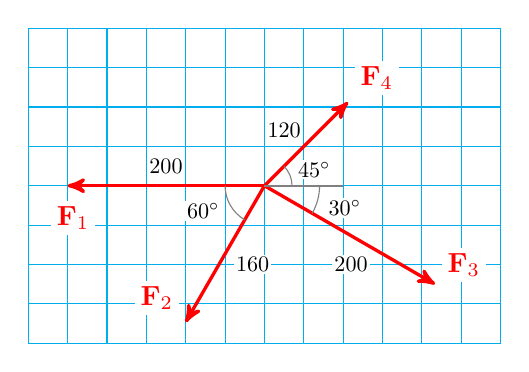
\begin{tikzpicture} [scale=.5]
\draw[cyan] (0,0) grid (12,8);

\coordinate(O) at (6,4);
\coordinate(f1) at (-5,0);
\coordinate(f2) at (240:4);
\coordinate(f3) at (-30:5);
\coordinate(f4) at (45:3);

\draw[red, very thick,->,>=stealth'] (O)--++(f1) node[below , xshift=2, yshift=-5, fill=white, inner sep = 2]{$\textbf{F}_1$};
\draw[red, very thick,->,>=stealth'] (O)--++(f2) node[above left, xshift=-2, yshift=2, fill=white, inner sep = 2]{$\textbf{F}_2$};
\draw[red, very thick,->,>=stealth'] (O)--++(f3) node[above right, xshift=2, fill=white, inner sep = 2]{$\textbf{F}_3$};
\draw[red, very thick,->,>=stealth'] (O)--++(f4) node[above right, xshift=2, yshift=2, fill=white, inner sep = 2]{$\textbf{F}_4$};
\node[scale=.8, fill=white, inner sep =1] at (3.5,4.5) {200};
\node[scale=.8, fill=white, inner sep =1] at (5.7,2) {160};
\node[scale=.8, fill=white, inner sep =1] at (8.2,2) {200};
\node[scale=.8, fill=white, inner sep =1] at (6.5,5.4) {120};
\draw[gray] (5,4) arc(180:240:1) node[left, midway, xshift=-3, yshift=-2, text=black, fill=white, inner sep = 1, scale=.8]{$60\degree$};
\draw[gray,thick] (O)--++(2,0);
\draw[gray] (6.7,4) arc(0:45:.7) node[right, midway, xshift=2, yshift=2, text=black, fill=white, inner sep = 1, scale=.8]{$45\degree$};
\draw[gray] (7.4,4) arc(0:-30:1.4) node[right, midway, xshift=3, yshift=-3, text=black, fill=white, inner sep = 1, scale=.8]{$30\degree$};

\end{tikzpicture}
\newline





\end{document}
